%-----------------------------------LICENSE------------------------------------%
%   This file is part of tikz_figures.                                         %
%                                                                              %
%   tikz_figures is free software: you can redistribute it and/or              %
%   modify it it under the terms of the GNU General Public License as          %
%   published by the Free Software Foundation, either version 3 of the         %
%   License, or (at your option) any later version.                            %
%                                                                              %
%   tikz_figures is distributed in the hope that it will be useful,            %
%   but WITHOUT ANY WARRANTY; without even the implied warranty of             %
%   MERCHANTABILITY or FITNESS FOR A PARTICULAR PURPOSE.  See the              %
%   GNU General Public License for more details.                               %
%                                                                              %
%   You should have received a copy of the GNU General Public License along    %
%   with tikz_figures.  If not, see <https://www.gnu.org/licenses/>.           %
%------------------------------------------------------------------------------%

% Use the standalone class for displaying the tikz image on a small PDF.
\documentclass[crop, tikz]{standalone}

% Import the tikz package to use for the drawing.
\usepackage{tikz}

% Packages used for decorating curves with arrows.
\usetikzlibrary{arrows.meta, decorations.markings}

% Begin the document.
\begin{document}

    % Begin the drawing.
    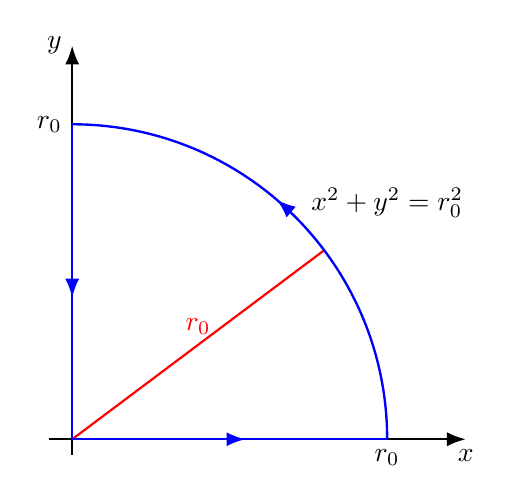
\begin{tikzpicture}[%
        line width = 0.3mm,
        > = Latex,
        ->-/.style = {
            decoration = {
                markings,
                mark = at position 0.55 with \arrow{>}
            },
            postaction = {decorate}
        }
    ]

        % Draw the coordinate axes.
        \draw[->] (-0.3, 0.0) to (5.0, 0.0) node [below] {$x$};
        \draw[->] (0.0, -0.2) to (0.0, 5.0) node [left] {$y$};

        % Line representing the radius of the circular arc.
        \draw[red, thick] (0.0, 0.0) to node [above] {$r_{0}$} (3.2, 2.4);

        % Three parts of the circular arc with arrows indicating direction.
        \draw[->-, blue] (0.0, 0.0) to (4.0, 0.0);
        \draw[->-, blue] (0.0, 4.0) to (0.0, 0.0);
        \draw[->-, blue] (4.0, 0.0) arc (0:90:4);

        % Labels for the axes and the circular arc.
        \node at (4.0, 3.0) {$x^{2}+y^{2}=r_{0}^{2}$};
        \node at (4.0, 0.0) [below] {$r_{0}$};
        \node at (0.0, 4.0) [left] {$r_{0}$};
    \end{tikzpicture}
\end{document}
